%  !TeX  root  =  user_guide.tex 

\section{Delimited Text Plugin}\label{label_dltext}    

% when the revision of a section has been finalized, 
% comment out the following line:
%\updatedisclaimer

The Delimited Text plugin allows you to load a delimited text file as a layer in QGIS. 

\minisec{Requirements}

To view a delimited text file as layer, the text file must contain:

\begin{enumerate}      
\item A delimited header row of field names. This must be the first line in the text file.
\item The header row must contain an X and Y field. These fields can have any name.
\item The x and y coordinates must be specified as a number. The coordinate system is not important.
\end{enumerate}

As an example of a valid text file we import the elevation point data file 
\filename{elevp.csv} coming with the QGIS sample dataset (See Section~\ref{label_sampledata}):

\begin{verbatim} 
X;Y;ELEV
-300120;7689960;13
-654360;7562040;52
1640;7512840;3
[...]
\end{verbatim}

Some items of note about the text file are:

\begin{enumerate}
\item The example text file uses \mbox{$;$} as delimiter. Any character can be used to delimit the fields.
\item The first row is the header row. It contains the fields X, Y and ELEV.
\item No quotes ({\tt{}"{}}) are used to delimit text fields.
\item The x coordinates are contained in the {\em X} field.
\item The y coordinates are contained in the {\em Y} field.
\end{enumerate}

\minisec{Using the Plugin}
To use the plugin you must first enable it as described in Section \ref{sec:managing_plugins}.

Click the new toolbar icon \toolbtntwo{delimited_text}{Add Delimited Text Layer} to open the Delimited Text dialog as shown in Figure \ref{fig:delim_text_plugin_dialog}.

\begin{figure}[ht]
   \centering
   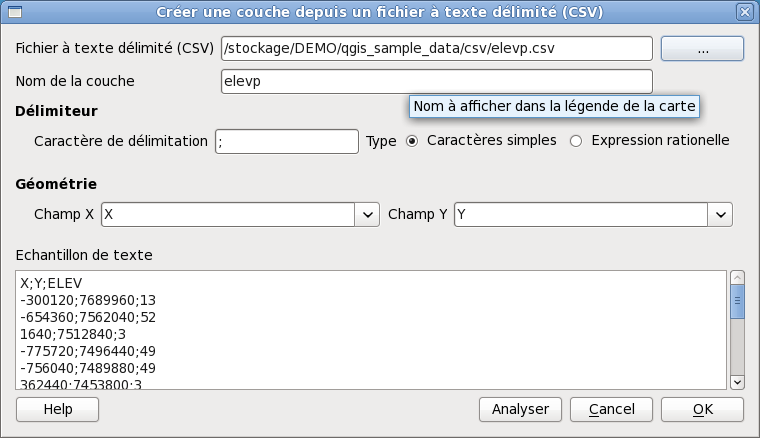
\includegraphics[clip=true, width=10cm]{delimited_text_dialog}   
   \caption{Delimited Text Dialog \nixcaption}\label{fig:delim_text_plugin_dialog}
\end{figure}

First select the file (e.g., \filename{qgis\_sample\_data/csv/elevp.csv}) to import by clicking 
on the \button{Browse} button. Once the file is selected, the plugin attempts to parse the file 
using the last used delimiter, in this case a semi-colon (\mbox{$;$}). To properly parse the file, it 
is important to select the correct delimiter. To change the delimiter to tab use 
\mbox{$\backslash$}t (this is a regular expression for the tab character).
After changing the delimiter, click \button{Parse}.

Once you have parsed the file, choose the X and Y fields from the drop down lists and 
enter a Layer name (e.g., \filename{elevp} ) as shown in Figure 
\ref{fig:delim_text_plugin_dialog}. To add the layer to the map, click 
\button{Add Layer}. The delimited text file now behaves as any other map layer in QGIS.

\FloatBarrier
